\chapter{Alignment}

One major hurdle in inferring neural structure from EM images is that the image acquisition process is inherently noisy. While the EM imaging technologies used for the creation of neuron images (typically TEM) are quite stable, there is often variance in sample preparation techniques, resulting in all sorts of distortions and errors at imaging time. One particular type of error, image misalignment, occurs during the slicing of sample tissue, when some physical factor causes a resulting slice to be warped or translated in such a way that the resulting stack of images is misaligned. Intuitively, this means that every point in one EM slice data does not necessarily map to the point directly below it the neighboring slice. An example of slice misalignment can be visualized in Figure \ref{fig:misalignment_example}.

\begin{figure}[h]
    \centering
	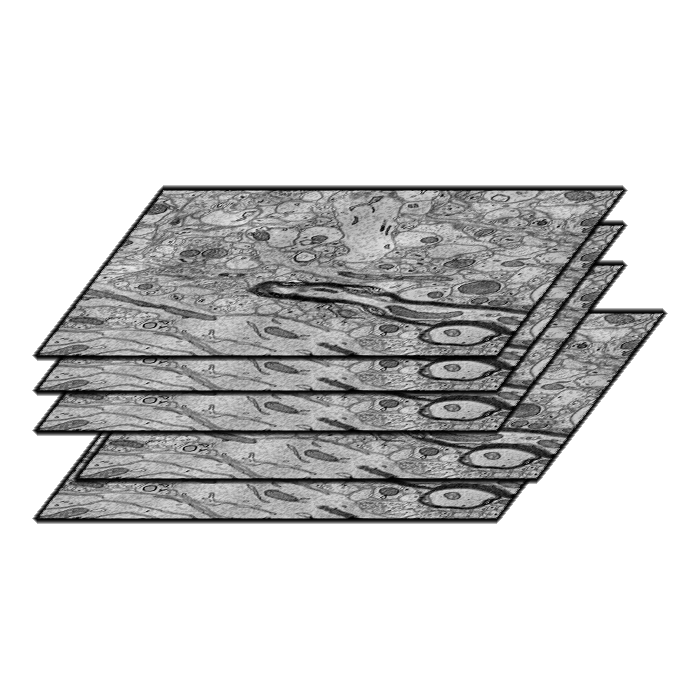
\includegraphics[width=0.33\textwidth]{img/misalignment_example}
	\hspace{1cm}
	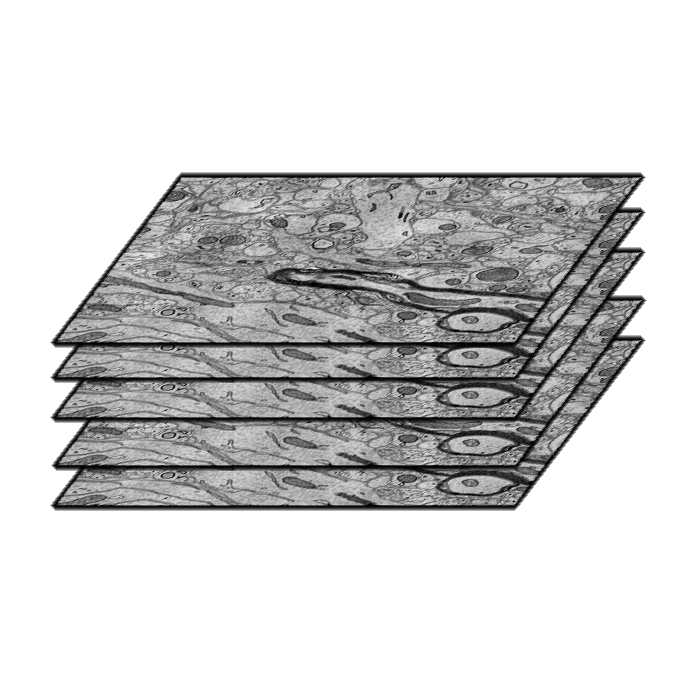
\includegraphics[width=0.33\textwidth]{img/alignment_example}
    \caption[An example of a 3D stack of EM images that contains a misalignment]{An example of a 3D stack of EM images that contains a misalignment. Left: The provided alignment of a stack. This represents a misalignment where the fourth image in a stack of images actually represents a slice slightly translated in position. Right: The correct alignment of the stack, where all the pixels in the fourth position have been translated enough such that the structures depicted in the input data line up in the z-direction.}
    \label{fig:misalignment_example}
\end{figure}

The problem of misalignment within a set of EM images particularly induces problems in the task of 3D Segmentation. While most techniques are rather invariant to small misalignments (particularly CNNs, which can be trained to be invariant to warping of many kinds), large misaligments can often induce false splitting in segmentations. Very deep CNNs trained with a really diverse set of data would likely be able to compensate for these sorts of misalignments, but it would be more prudent to develop a more efficient strategy for automatically healing misalignments in the data. 

In this section, we will define the task of realignment, construct and train models, and examine the results of these experiments. 


\section{Task Definition}

In an abstract sense, the realignment task is to take a stack of raw EM images and distort it such that it as accurately as possible reflects the reality of the underlying biological structures it supposedly represents. This is a bit too daunting of a task for the scope of this paper, so instead propose the task of realigning one 'distorted' slice to another 'reference' slice, with the stipulation that these two slices are adjacent within some EM stack. That is, transform one of two consecutive images in an EM stack such that their aligment is maximized.

\section{Evaluation Metrics}

Coming up with an empirical metric to measure the aligment of two images is difficult, because domain-knowledge is required to say with certainty whether two images are probably aligned. So, in lieu of a metric for alignment, we will take an already aligned (i.e. by the empirical methods mentioned in Chapter 1) stack of images and randomly distort them. Both the parameters for distortion (which can be any sort of parameterized transform) and the original, undisturbed image of the 'distorted' slice can serve as labels when evaluating error, since the distortions were induced.

From this formulation, we define three evaluation metrics, all of which are defined in Appendix A:
\begin{itemize}
	\item \textbf{Pixel Error}: We will use Pixel Error to determine whether, when given a correctly-aligned 'reference' image and a 'distorted' image, the model outputs an image that is pixelwise close to the preimage of the 'distorted' image.
	\item \textbf{Cross Correlation}: Similar to Pixel Error, we will use Cross Correlation to determine whether or not a model's prediction aligns with the preimage of a 'distorted' image. Cross Correlation is somewhat more continuous than Pixel Error.
	\item \textbf{L2 Error on Parameters}: The parameters to a transformation are typically continuous real numbers, meaning that we can calculate a meaningful L2 Error on the Parameters if our model predicts a set of parameters (rather than simply predicting the set of images).
\end{itemize}

\section{Models}

\begin{figure}
\centering
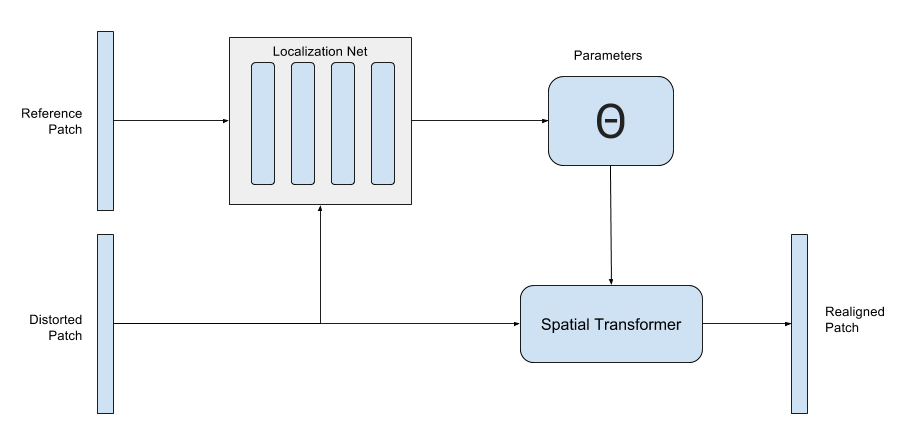
\includegraphics[width=\textwidth]{img/Spatial_Transformer.png}
\caption[A prototypical Spatial Transformer Network]{A prototypical Spatial Transformer Network. The major components of the network are the localization net, and the spatial transformer module. Both sections are fully differentiable, meaning that a gradient can be backpropogated through the transform and up through the localization net for training.}
\label{fig:spatial_transformer}
\end{figure}

Both of our models for predicting realignment are based on the Spatial Transformer Network, which was originally designed as a tool to regularize convolutional networks and speed up image classification tasks\cite{Jaderberg2015}. Spatial Transformer Networks are conceptually straightforward: it is possible to define a class of image transformations (i.e. rotation, translation, affine) that are at least partially differentiable. If a transformation is at least partially differentiable, then any gradient that is calculated at the output of the transformer can be backpropogated through the transformer and into its parameters. This means that parameters can be learned, through the use of a localization net. In general, for a chosen spatial transform (a sub-differentiable transform), localization nets can take on any architecture that produce appropriate parameters for that transformer. We define two models; for both we will choose as our spatial transformer module the affine transform\footnote{An affine transform is a class of transforms that include rotation, scaling, shearing, and translating. An affine transform is parameterized by 6 real numbers.} module as outlined in the original paper. Our two localization models are:

\begin{itemize}
	\item \textbf{Fully Connected}: The Fully Connected (FC) localization network is a shallow attempt at learning simple transformations. For a pair of fixed size images with $N$ pixels (the 'reference' image and the 'distorted' image), the FC localization network has two fully connected layers, with 512 units in the first layer, and 6 units in the last layer. We apply ReLU between the first and second layer, and because the parameters of an affine transform can be negative or positive, the final layer is run through a tanh function before being output.
	
	\item \textbf{Standard Convolutional}: The Standard Convolutional localization network has the same set of outputs and inputs as the FC localization network, namely taking two $N$-sized inputs, and outputting 6 parameters. The network consists of 4 convolutional layers, each with 3 (1x3x3) convolutions into 48 feature maps, a ReLU nonlinearity, and a (1x2x2) pooling. After these four layers are two fully connected layers, that work in the same way as in the FC localization net, except with inputs that match the outputs of the last pooling. 
\end{itemize}

Both these models were chosen because of examples in the original Spatial Transformer paper. Future work will likely consist of designing alternate architectures.


\section{Dataset}

For simplicity, we use the ISBI 2012 dataset referenced in Chapter 3. This dataset is quite well-aligned, and serves as a good ground-truth for random misalignments to be applied to. Just as before, a validation set was held out from the training set to give us a way to evaluate our performance.

\section{Training}

We trained our models for 100,000 steps each, randomly sampling a pair of adjacent patches from the dataset and applying a random translation or rotation to both patches, designating one patch as the 'reference' patch and the other the 'distorted' patch. A third 'ground truth' patch is calcuated by taking the preimage of the 'distorted' patch and applying the same transformation as was applied to the 'reference' patch. This creates a training input and label. Both translation and rotation were bounded to within realistic values for the problem domain (i.e. so that images weren't offset by twice their length).

We attempted to train each of our models under various conditions: without augmentation on the dataset, and with augmentation on the dataset when sampled. That is, we either drew from a very small training set, or a very large one. 

We attempted to use two different loss functions: smoothed cross correlation, and L2 Loss on the parameters. The smoothed cross correlation was calculated after the predicted transformation was applied, but because both of our model types predicted parameters for a transformation using a Spatial Transformer, we were able to backpropogate the gradient for this loss function back through the Spatial Transformer and into the predicted parameters.

\section{Results}

Unfortunately, we found that our quantitative results were not of sufficient quality to report. We found that when training both styles of localization nets without augmentation the nets would actually learn how to compensate for arbitrary translations and rotations on data it had seen before. That is, if it saw a pair of patches it had seen before, but not necessarily with the particular transformation, it could heal that never-before-seen transformation. However, there was no generalization whatsoever when testing on the validation set: predictions were effectively random. This occured for all of our models, regardless of whether we trained with the pre-transformation parameters as our label or with the transformed image as our label.

Despite these discouraging results, we believe that this particular avenue for exploration has promise. Because we were able to train nets that could learn arbitrary transformations on image data it had seen before, we believe that the primary impediment is localization net architecture, rather than the whole Spatial Transformer concept. Perhaps a deeper or wider net would show improvements, or one with residual connections to maintain the original features of the 'distorted' image. 

Additionally, one of the key properties of the Spatial Transformer Network is that it can propogate gradients from downstream tasks through the transformation layer. This could potentially allow for a segmentation model that, instead of learning based ona fixed alignment, dynamically learns an alignment such that segmentation accuracy is directly maximized.